% !TEX root = ../set_recommendation.tex
\begin{figure*}[t!]
  \centering
%  \pdfimageresolution=500  
  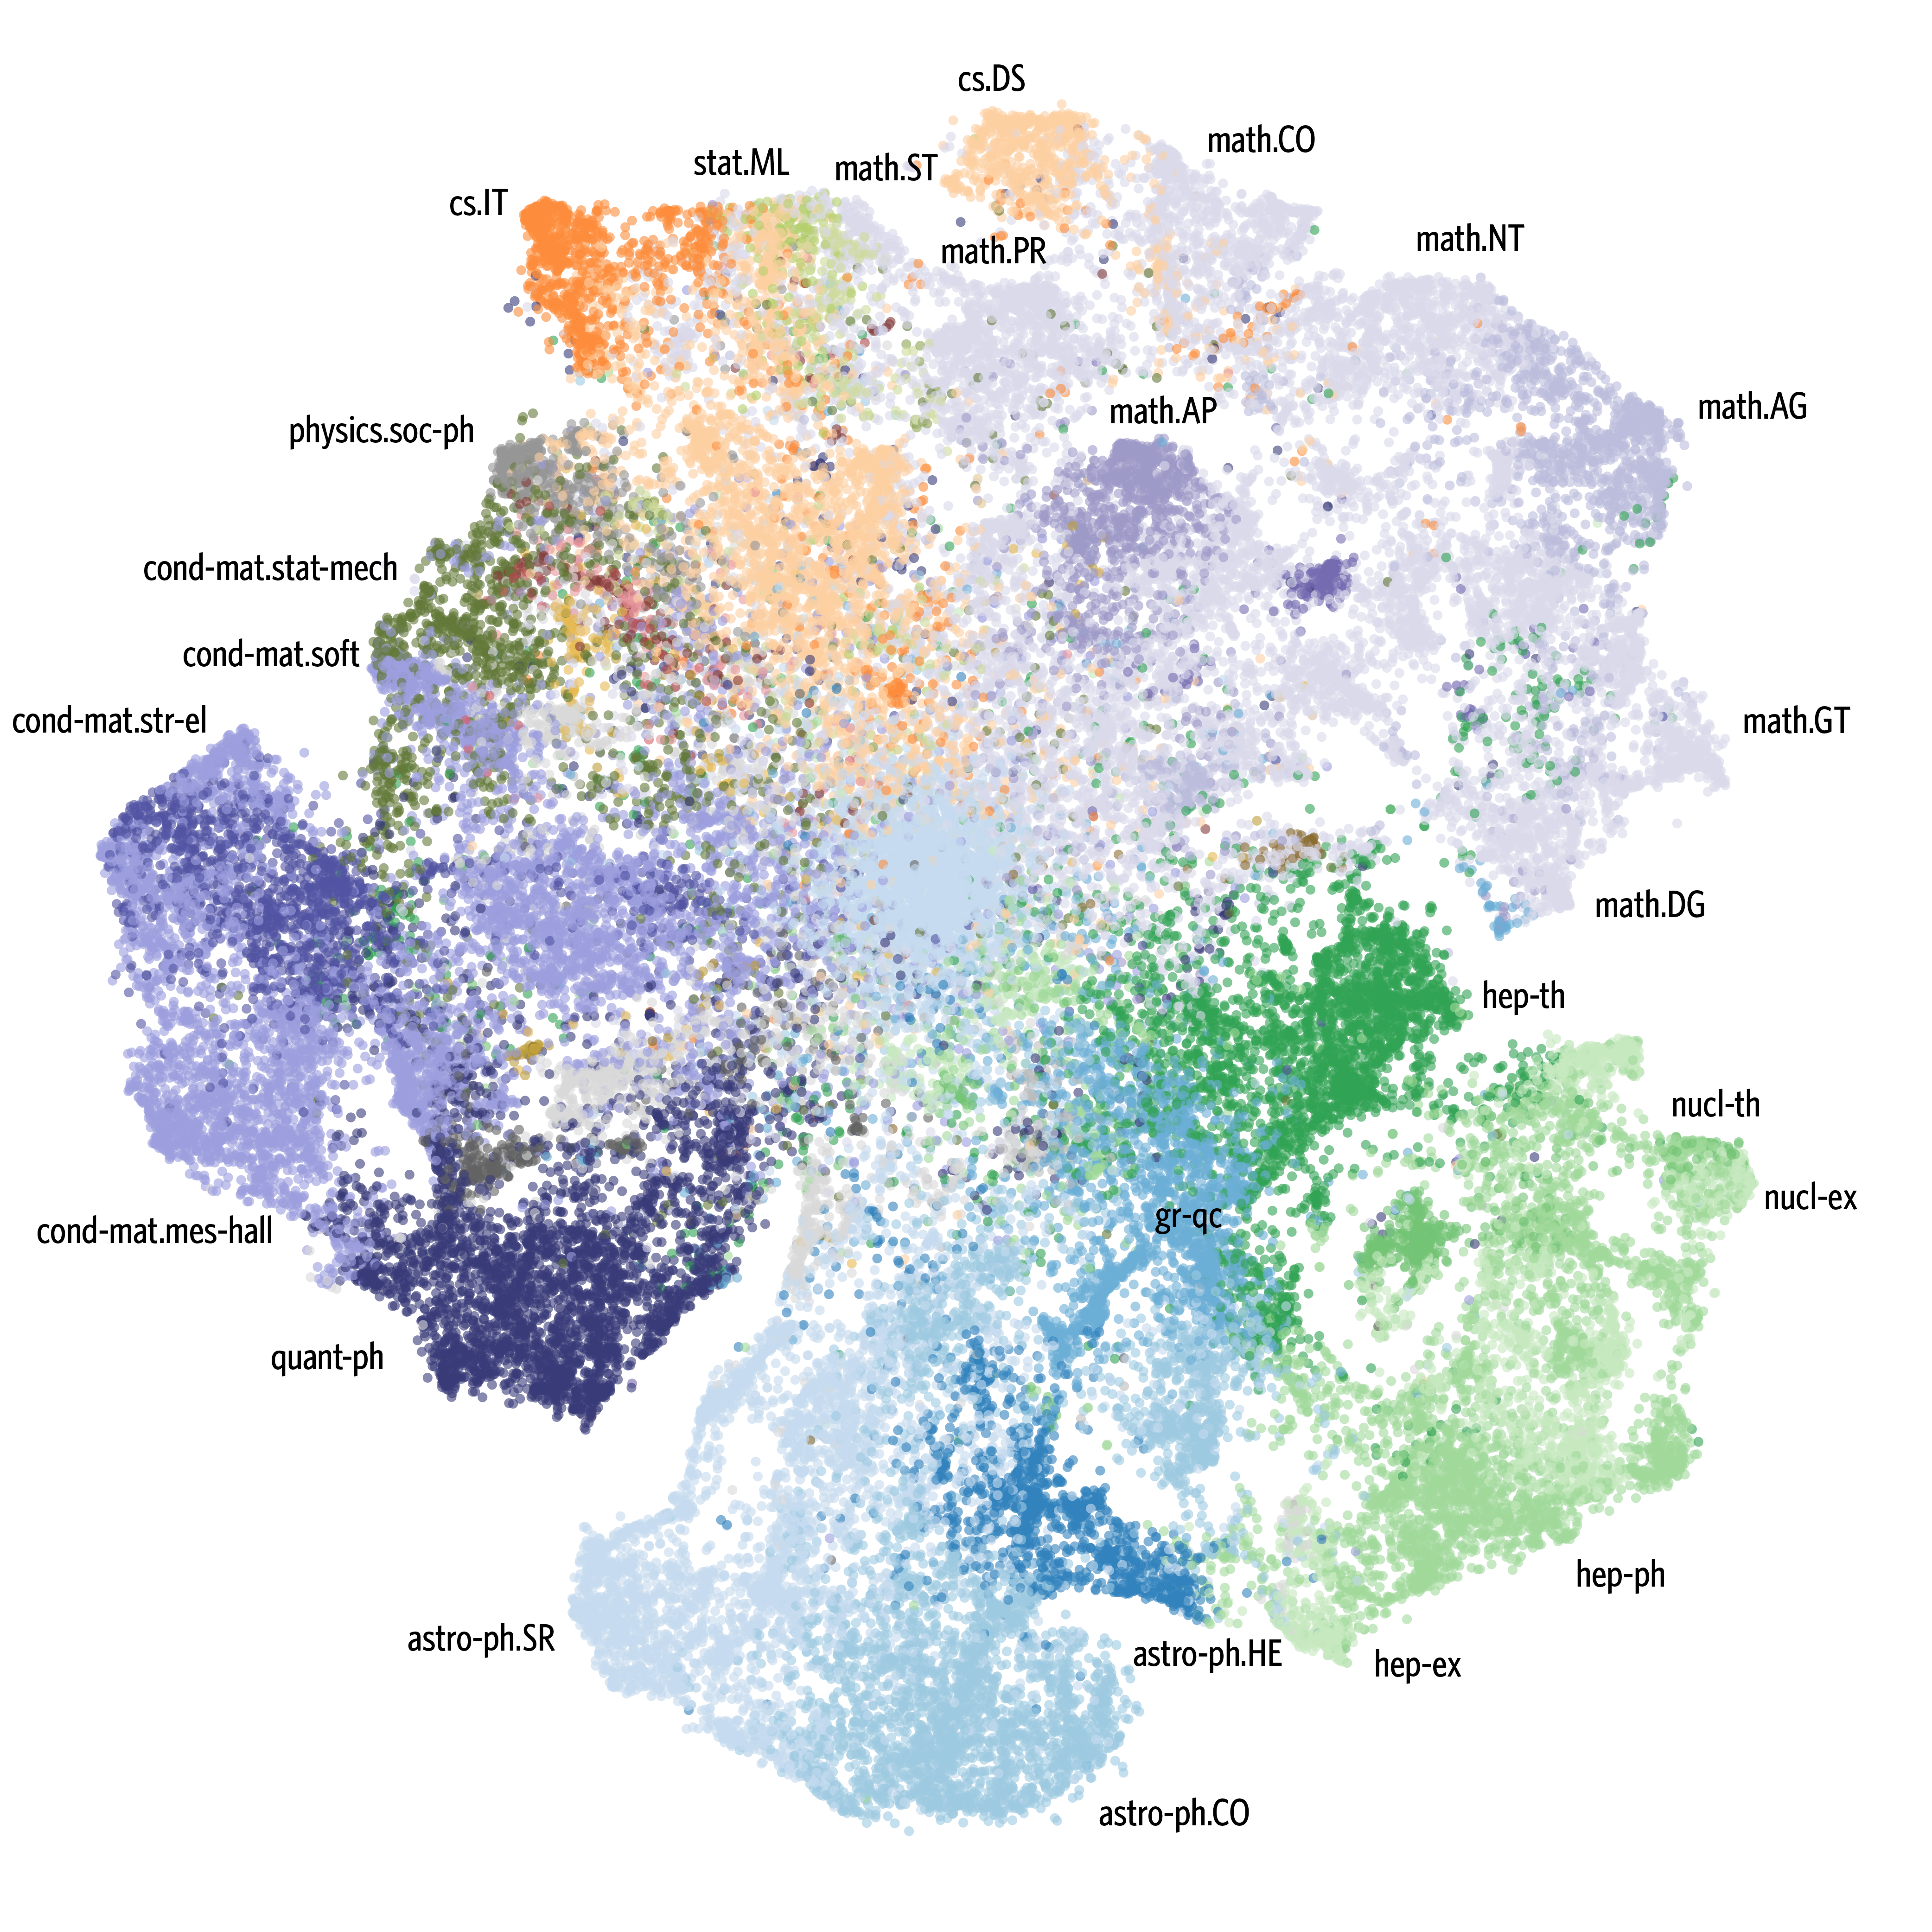
\includegraphics[width=0.95\textwidth]{fig/arxiv_user_embeddings_tsne.png}
  \caption{\label{fig:arxiv_tsne} \acrlong{rfs} trained on arXiv reading
    behavior clusters researchers by their most frequently-read arXiv category
    (best viewed in color). On this data, \acrlong{rfs} is trained to recommend
    items using their attributes as described in \Cref{sec:experiments_arxiv};
    the set of attributes for a paper is the set of words in the abstract. A
    visualization of the user embeddings in the inner product regression
    function in \Cref{eqn:rankfromsets} yields an interpretable map of science.
    We use the t-SNE algorithm~\citep{maaten2008visualizing} for visualizing the
    high-dimensional embeddings in two dimensions. In this map of science,
    fields of study are related according to patterns in how people read papers
    in neighboring fields. Each marker represents a user embedding; the color
    assigned to a user is determined the user's most-read arXiv category. The
    color assigned to a category is determined by the most-read categories
    across the arXiv, with similar colors assigned to similar fields according
    to the arXiv ontology. For an interactive version of this map, please visit
    anon-url which enables zoom and display of all 143 arXiv category labels to
    explore the relationships between different fields of science.}
\end{figure*}


%%% Local Variables:
%%% mode: latex
%%% TeX-master: "../set_recommendation"
%%% End:
